\section{Real-Time System (Echtzeitsystem)}

\subsection{Definitionen}

\subsubsection{Real-Time System (Echtzeitsystem)}

\begin{itemize}
    \item Ein Echtzeitsystem ist ein System, das Informationen \textbf{innerhalb einer definierten Zeit (deadline) bearbeiten} muss. \\
        \textrightarrow\ Explizite Anforderungen an \textbf{turnaround-time} (Antwortzeit) müssen erfüllt sein
    \item Wenn diese Zeit nicht eingehalten werden kann, ist mit einer \textbf{Fehlfunktion} zu rechnen.
\end{itemize}

\vspace{0.2cm}

\begin{minipage}[t]{0.55\columnwidth}
    \begin{center}
        \myul{\textbf{Typisches Echtzeitsystem}}

        \vspace{0.1cm}

        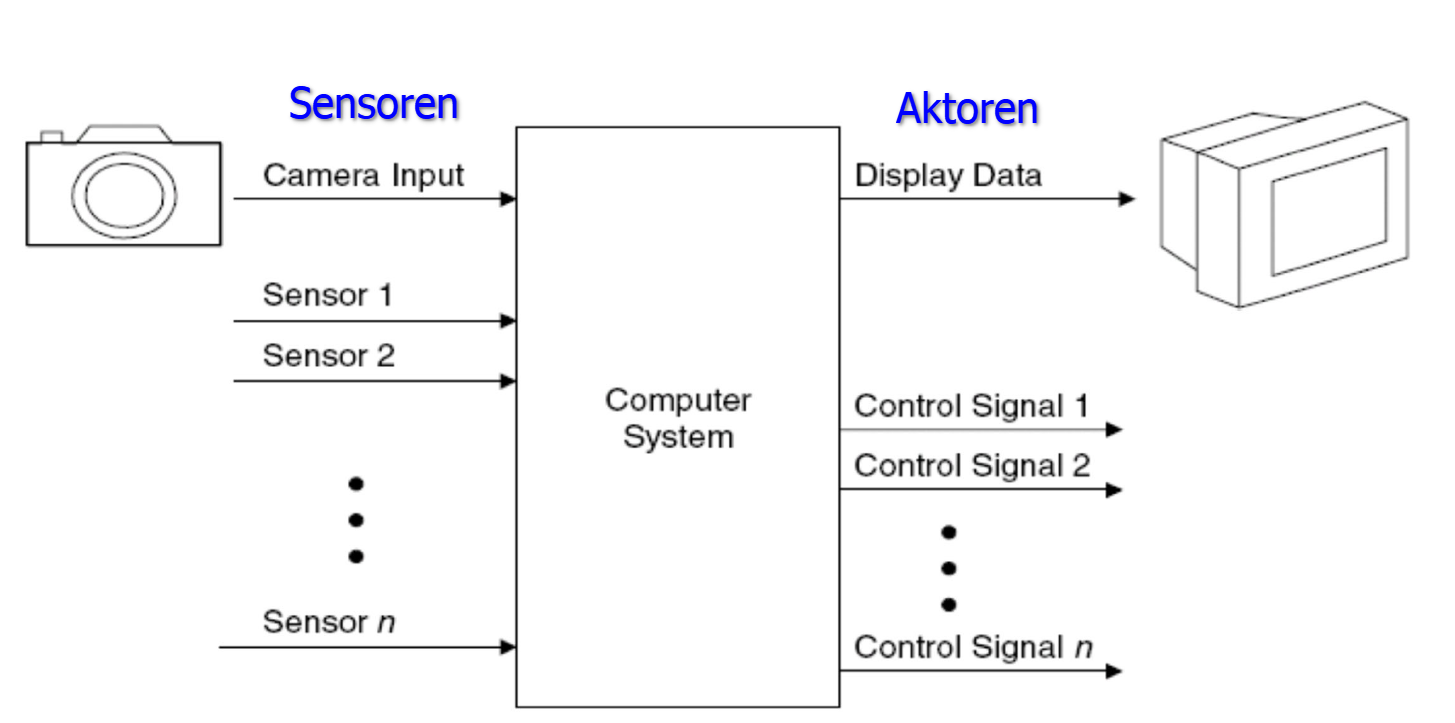
\includegraphics[width=\columnwidth]{images/typisches_echtzeitsystem.png}
    \end{center}
\end{minipage}
\hfill
\begin{minipage}[t]{0.4\columnwidth}
    \begin{center}
        \myul{\textbf{Repräsentation RT-System}}

        \vspace{0.1cm}

        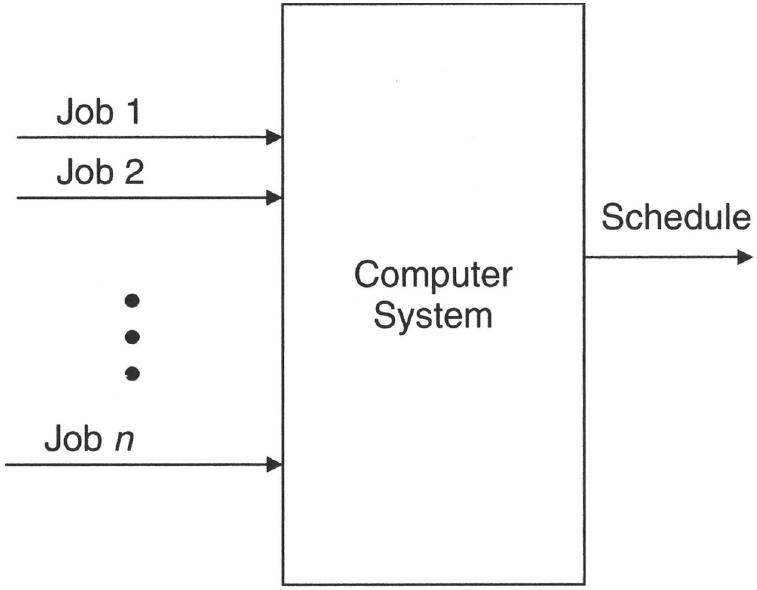
\includegraphics[width=0.7\columnwidth]{images/typische_repraesentation_echtzeitsystem.png}

        Sequenz von Aufgaben (Jobs) müssen zeitlich geplant (scheduled) werden
    \end{center}
\end{minipage}



\subsubsection{Zeitdefinitionen (Task)}

\begin{center}
    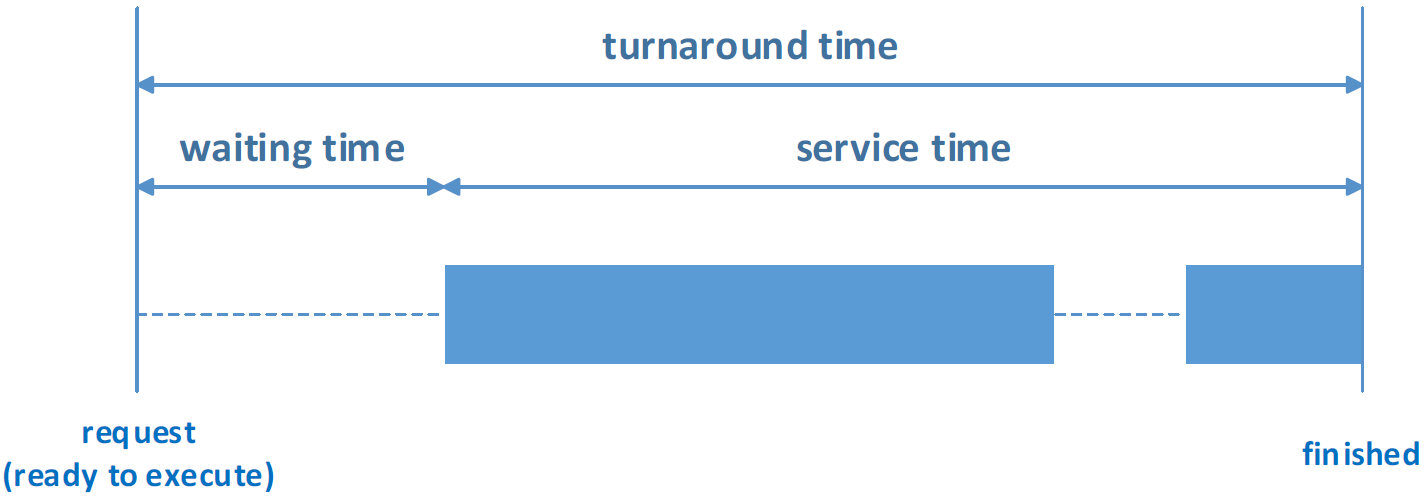
\includegraphics[width=0.7\columnwidth]{images/zeitdefinitionen_task.png}
\end{center}

\begin{outline}
    \1 \textbf{turnaround time:} (response time, Antwortzeit) 
        \2 Startet, wenn der Task bereit zur Ausführung ist und endet, wenn der Task fertig abgearbeitet ist
        \2 Zeit zwischen dem Vorhandensein von Eingangswerten an das System (Stimulus) bis zum Erscheinen der gewünschten Ausgangswerte.
    \1 \textbf{waiting time:} (Wartezeit)
        \2 Zeit zwischen Anliegen der Eingangswert und Beginn der Abarbeitung des Tasks
    \1 \textbf{service time:} (Bearbeitungszeit)
        \2 Zeit für Abarbeitung des Tasks \textrightarrow\ Unterbrechungen bzw. (preemptions) möglich 
\end{outline}


\subsection{Fehlverhalten eines Systems (failed system)}

\begin{itemize}
    \item Ein fehlerhaftes System (failed system = missglücktes System) ist ein System, das nicht alle formal
        definierten Systemspezifikationen erfüllt.
    \item \textbf{Die Korrektheit eines RT Systems bedingt sowohl die Korrektheit der Outputs als auch die Einhaltung
        der zeitlichen Anforderungen.}
\end{itemize}


\subsection{Echtzeitdefinition -- Verschiedene Echtzeitsysteme}

\begin{outline}
    \1 \textbf{soft real-time system} (weiches Echtzeitsystem)
        \2 Durch Verletzung der Antwortzeiten wird das System \textbf{nicht} ernsthaft beeinflusst
        \2 Es kommt zu Komforteinbussen
    \1 \textbf{hard real-time system} (hartes Echtzeitsystem)
        \2 Durch Verletzung der Antwortzeiten wird das \textbf{System ernsthaft beeinflusst}
        \2 Es kann zu einem kompletten Ausfall oder katastrophalem Fehlverhalten kommen
    \1 \textbf{firm real-time system} (festes Echtzeitsystem)
        \2 Kombination aus soft real-time system und hard real-time system
        \2 Durch Verletzung einiger weniger Antwortzeiten wird das System nicht ernsthaft beeinflusst
        \2 Bei vielen Verletzungen der Antwortzeiten kann es zu einem kompletten Ausfall oder katastrophalem Fehlverhalten kommen
\end{outline}


\subsubsection{Beispiele verschiedener Echtzeitsysteme}

\begin{center}
    \begin{tabular}{@{}lll@{}}
        \toprule
        \textbf{System}     & \textbf{Klassifizierung}  & \textbf{Erlärung}                             \\
        \midrule
        Geldautomat         & soft                      & Auch wenn mehrere Deadlines nicht eingehalten \\
                            &                           & werden können, entsteht dadurch keine         \\
                            &                           & Katastrophe. Im schlimmsten Fall erhält ein   \\
                            &                           & Kunde sein Geld nicht.                        \\
        \midrule
        GPS-gesteuerter     & firm                      & Wenn die Positionsbestimmung versagt, könnte  \\
        Rasenmäher          &                           & das Blumenbeet der Nachbarn platt gemäht      \\
                            &                           & werden.                                       \\
        \midrule
        Regelung eines      & hard                      & Das Versagen der Regelung kann dazu führen,   \\
        Quadrocopters       &                           & dass der Quadrocopter ausser Kontrolle        \\
                            &                           & gerät und abstürzt.                           \\
        \bottomrule
    \end{tabular}
\end{center}


\subsection{Determinsismus (determinacy)}

Ein System ist deterministisch, wenn für jeden möglichen Zustand und für alle möglichen Eingabewerte
\textbf{jederzeit der nächste Zustand und die Ausgabewerte definiert} sind.

\vspace{0.2cm}

Insbesondere race conditions können dazu führen, dass der nächste Zustand davon abhängt, 'wer das
Rennen gewonnen hat und wie gross die Bestzeit ist', d.h. der nächste Zustand ist nicht klar bestimmt.\\
\textrightarrow\ Nicht mehr deterministisch und nicht mehr echtzeittauglich


\subsection{Auslastung (utilization)}

Die (CPU-) Auslastung (utilization) ist der Prozentsatz der Zeit, zu der die XPU \textbf{nützliche (non-idle) Aufgaben} ausführt. 


\subsubsection{Berechungen zur Auslastung (utilzation)}

\textbf{Annahmen:}

\begin{itemize}
    \item System mit $n \geq 1$ periodischen Tasks $T_i$ und Periode $p_1$
    \item Jeder Task $T_i$ het bekannte / geschätzte maximale (worst case) execution time $e_i$
\end{itemize}

\vspace{0.2cm}

\begin{minipage}[t]{0.48\columnwidth}
    \begin{center}
        \myul{\textbf{Auslastungsfaktor eines Tasks}}
        $$ u_i = \frac{e_i}{p_i} $$
        \textrightarrow\ utilization factor
    \end{center}
\end{minipage}
\hfill
\begin{minipage}[t]{0.48\columnwidth}
    \begin{center}
        \myul{\textbf{Gesamtauslastung des Systems}}
        $$ U = \sum\limits_{i=1}^n u_i = \sum\limits_{i=1}^n \frac{e_i}{p_i} $$
        \textrightarrow\ utilization
    \end{center}
\end{minipage}

\vspace{0.2cm}
\textrightarrow\ Bei 69 \% Auslastung ist das  \textbf{'theoretical limit'} % CHECK Mehr dazu folgt später im Semester


\subsection{Real-time Scheduling}

\begin{outline}
    \1 Alle kritischen Zeiteinschränkungen (deadlines, response time) sollen eingehalten werden
    \1 Im Notfall muss der Scheduling Algorithmus entscheiden, um die kritischsten Tasks einhalten zu können.
        \2 Unter Umständen müssen dabei Deadlines von weniger kritischen Tasks verletzt werden.
\end{outline}

